\documentclass{beamer}
\usepackage{../preamble/custom}

\setbeamertemplate{bibliography item}[text]

\title{Maximal repetition \& ``Runs'' conjecture}
\author{Riccardo Lo Iacono \\ \footnotesize{Docente: Gabriele Fici}}
\begin{document}
    \begin{frame}
        \maketitle
    \end{frame}

    \begin{frame}{Notazione}
        \begin{itemize}
            \item \(\Sigma\) è un alfabeto ordinato e finito di simboli
            \item Un elemento \(S \in \Sigma^{*}\) è detto stringa,
                la cui lunghezza è denotata da \(\abs{S}\)
            \item L'i-esimo carattere di S sarà denotato da S[i],
                \(1 \le i \le n = \abs{S}\)
            \item Per ogni i, j S[i, j] indica la sottostringa compresa tra le 
                posizioni i e j, \(1 \le i \le j \le n = \abs{S}\)
        \end{itemize}
    \end{frame}

    \begin{frame}{Periodo ed esponente}
        \textbf{Definizione: } Data S una stringa,
        si definisce \emph{periodo} un intero \(p \ge 1\)
        tale che S[i] = S[i + p], \(\forall i = 1, \ldots, \abs{S} - p\)

        \textbf{Definizione: } Si definisce \emph{esponente} \(\exp\)
        il rapporto tra la lunghezza di S e del suo più piccolo periodo.
    \end{frame}

    \begin{frame}{Ripetizioni massimali}
        \textbf{Definizione: } Una coppia (i, j) è detta ripetizione massimale
        (o run) di una stringa S, se \(\exp\{S[i, j]\} \ge 2p\) e la periodicità
        non può essere estesa ne a destra ne a sinistra.

        Sia \emph{Runs\{S\}} l'insieme dei run in S, 
        \(\rho(S)\) la sua cardinalità.
    \end{frame}

    \begin{frame}{Un esempio}
        Sia considerata la stringa \(S = babbabbababbabbabc\) che contiene nove 
        run, mostrati in \emph{Figura \ref{fig:1}}.

        \begin{figure}[!h]
            \centering
            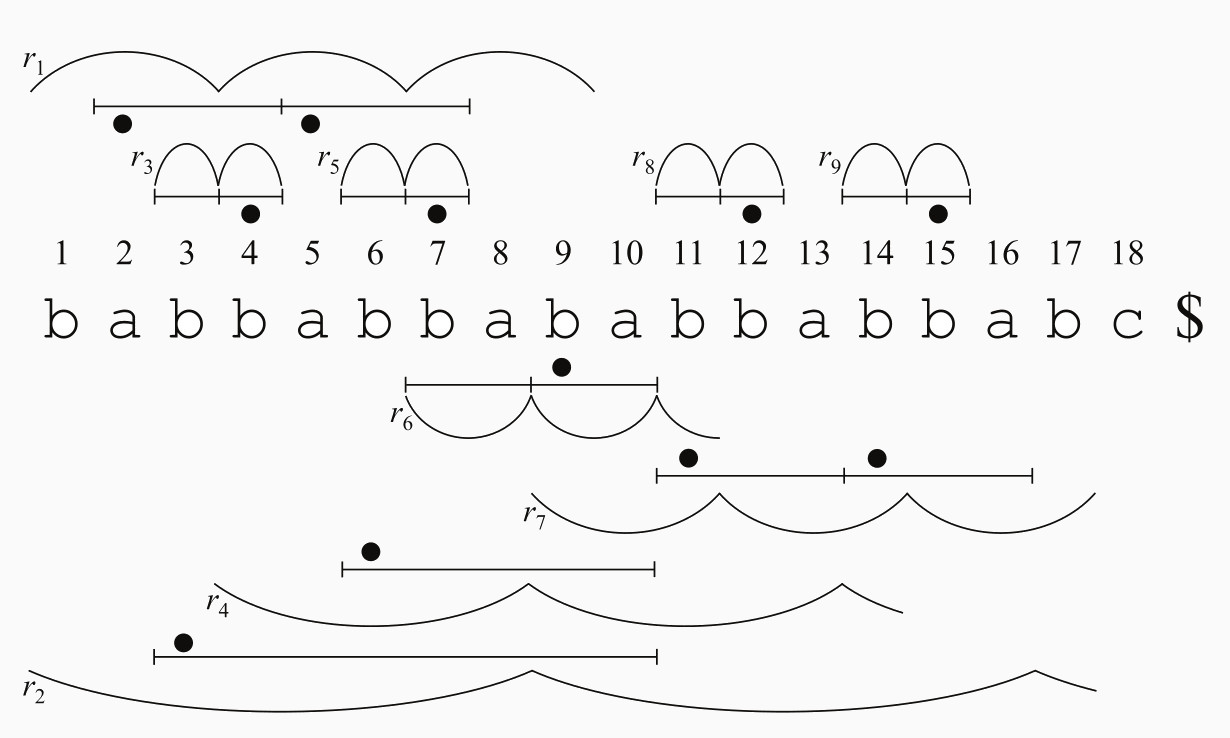
\includegraphics[scale = .85]{../Extra/run example.jpg}
            \caption{Illustrazione run nella stringa S = babbabbababbabbabc.}
            \label{fig:1}
        \end{figure}
    \end{frame}

    \begin{frame}{Background storico}
        \emph{Kolpakov \emph{e} Kucherov}\footnotemark[1]
        dimostrano che \(\rho(S) = \bigO{|S|}\).
        \vskip 10pt
        \textbf{Congettura (Runs conjecture):} \(\rho (S) < |S|\) per ogni stringa S.

        \footnotetext[1]{R. M. KUCHEROV {\footnotesize AND} G. KOLPAKOV,
                 \emph{Finding maximal repetitions in a word in linear time. FOCS, 1999}
         }
    \end{frame}

    \begin{frame}{Punti chiave della discussione}
        \begin{itemize}
            \item Dimostrazione della runs conjecture.
            \item Soluzione algoritmica per il calcolo delle ripetizioni 
                massimali in \(\bigO{n}\).
        \end{itemize}
    \end{frame}
    
    % \begin{frame}
    %     \textbf{Esempio: } sia \(s = babbabbab\).
    %     Si osserva facilmente che le ripetizioni massimali in essa sono quelle 
    %     in \emph{Figura \ref{fig:1}}.
    %     \begin{figure}[!h]
    %         \centering
    %         \begin{tikzpicture}
    %             \foreach \char/\i in {b/0, a/1, b/2, b/3, a/4, b/5, b/6, a/7, b/8} {
    %                 \node at (\i, 0) {\char};
    %             }    
    %
    %             \draw[ |-| ] (2, .5) -- (3, .5); 
    %
    %             \draw[ |-| ] (5, .5) -- (6, .5);
    %
    %             \draw[ |-| ] (0, -.5) -- (2.5, -.5);
    %             \draw[ -| ] (2.5, -.5) -- (5.5, -.5);
    %             \draw[ -| ] (5.5, -.5) -- (8, -.5);
    %
    %             \node at (2.5, .5) [anchor =south] {\(r_{2}\)};
    %             \node at (5.5, .5) [anchor = south] {\(r_{3}\)};
    %             \node at (0, -.5) [anchor = east] {\(r_{1}\)};
    %
    %         \end{tikzpicture}
    %         \caption{Esempio di ripetizioni massimali}
    %         \label{fig:1}
    %     \end{figure}
    %     Segue che 
    %         \[
    %             Runs(babbabbab) = \{(1, 9, 3), (3, 4, 1), (6, 7, 1)\} 
    %         \]
    % \end{frame}
    %
    % \begin{frame}{Lyndon words \&  L-roots}
    %     \textbf{Definizione} (Lyndon word): una stringa non vuota \(s \in \Sigma^{*}\)
    %     è detta essere una \emph{Lyndon word}, rispetto a \(\prec\), 
    %     se \(s \prec u\), per ogni \(u\) suffisso proprio di \(s\).
    %     \vskip 5pt
    %      Definizione equivalente è la seguente:
    %     \vskip 5pt
    %     \textbf{Definizione: } data una stringa \(s\) di lunghezza \(n\) e 
    %     \(i \in [1, n]\), la stringa \(s_{i}s[1, i - 1]\) è detta 
    %     \emph{shift ciclico} di \(s\), non banale se \(i > 1\).
    %     Una Lyndon word è una stringa non vuota che è lessicograficamente minore
    %     di ogni suo shift ciclico non banale.
    %     \vskip 10pt 
    %     \textbf{Definizione} (L-root): dato \(r = (i, j, p)\) un run per una 
    %      stringa \(s \in \Sigma^{*}\),
    %     un intervallo \(\lambda = [i_{\lambda}, j_{\lambda}]\) è detto essere
    %     \emph{L-root} di \(r\) rispetto a \(\prec\) se 
    %     \(i \le i_{\lambda} \le j_{\lambda} \le j\)
    %     e \(s[i_{\lambda}, j_{\lambda}]\) è una Lyndon word.
    % \end{frame}
    %
    % \begin{frame}{``Runs'' Theorem}
    %     Sia \(\hat{s} = s\textdollar, \textdollar \notin \Sigma\).
    %     % Prima osservazione è che: se consideriamo la più lunga Lyndon word,
    %     % rispetto \(\prec_{0} \text{e} \prec{1}\) che inizia a un dato \(i\),
    %     % uno dei due avrà lunghezza 1.
    %
    %     \textbf{Lemma 1:} Per ogni stringa \(s\) e posizione \(i\),
    %     sia \(\ell \in \{0, 1\} \), tale che \(\hat{s}[k] \prec_{\ell} 
    %     \hat{s}[i], \text{per } k = \min \{ k' \, \vert \, \hat{s}[k'] \ne 
    %     \hat{s}[i], k' > i\}\). Allora \(l_{\ell}(i) = [i, i]\) e 
    %     \(l_{\overline{\ell}}(i) = [i, j], \text{per qualche } j > i\).
    %     \vskip 10pt 
    %     % Seconda osservazione è che: data una ripetizione \(r\),
    %     % esiste un ordine \(\prec_{\ell_{r}} \in \{\prec_{0}, \prec_{1}\}\)
    %     % tale che la L-root della runc rispetto \(\prec_{\ell_{r}}\)
    %     % coincide con la longest Lyndon word rispetto \(\prec_{\ell_{r}}\)
    %     % che inizia in quella posizione.
    %     \textbf{Lemma 2: } Sia \(r = (i, j, p)\) una ripetizione massimale in una stringa
    %     \(s\), sia inoltre \(\ell_{r} \in \{0, 1\}\) tale che 
    %     \(\hat{s}[j + 1] \prec_{\ell_{r}} \hat{s}[j + 1 -p]\).
    %     Allora, ogni L-root \(\lambda = [i_{\lambda}, j_{\lambda}]\) di \(r\)
    %     rispetto \(\prec_{\ell_{r}}\) è uguale a \(l_{\ell_{r}}(i_{\lambda})\).
    % \end{frame}
    %
    % \begin{frame}
    %    Sia \(B_{r}\) l'insieme delle L-root tali da soddisfare \emph{Lemma 2},
    %    allora vale quanto segue.
    %
    %    \textbf{Lemma 3: } per ogni coppia di ripetizioni massimali \(r, r'\), 
    %    con \(r \ne r'\), \(Beg(B_{r}) \cap Beg(B_{r'}) = \varnothing\).
    %
    %    Da ciò, poiché 
    %    \[
    %        \abs{Beg(B_{r})} = \abs{B_{r}} \ge \floor{e_{e} - 1} \ge 1
    %    \]
    %    e inoltre, dato che \(1 \notin Beg(B_{r})\) per ogni run \(r\), vale
    %    \(\sum_{r \in Runs(s)}{\abs{B_{r}}} = \sum_{r \in Runs(s)}{\abs{Beg(B_{r})}}
    %    \le \abs{s} - 1\).
    %
    %    \textbf{Teorema: } \(\rho(s) < n\).
    % \end{frame}
    %
    % \begin{frame}{L'algoritmo (Bannai et al.)} 
    %     Bannai et al. propongono un algoritmo per determinare le ripetizioni
    %     massimali; algoritmo che risulta però \(\Theta(n)\) (costo dipendente dal computo degli LCE).
    % \end{frame}
    %
    % \begin{frame}{osservazioni teoriche}
    %     Kosolobov ha dimostrato che, dato un generico alfabeto ordinato,
    %    si possono calcolare \(\bigO{n}\) LCE  in tempo 
    %     \(\bigO{n \log^{2\slash 3} n}\); congetturando l'esistenza di un 
    %     algoritmo lineare. \footnote{D. Kosolobov, Title, venue.}
    %
    %     Crochemore et al. hanno dimostrato che per computare \(\bigO{n}\) LCE 
    %     non sovrapposti è richiesto tempo \(\bigO{n \alpha(n)}\) (\(\alpha\) 
    %     funzione inversa di Ackermann) \footnote{M. Crochemore, Title, venue.}.
    % \end{frame}
    %
    % \begin{frame}
    %     \textbf{Definizione } (Next Smallest Suffix): 
    %     data \(s\) una stringa di lunghezza \(n\),
    %     il suo next-smallest-suffix (NSS) array è definito come segue:
    %     \[
    %         \forall i \in [1, n],  nss[i] = \min\{j \mid j = n + 1 \lor 
    %             (j \in (1, n] \land s[i, n] \succ s[j, n])\}
    %     \]
    %     Se \(nss[i] \le n, s[nss[i], n]\) è detto next-smallest-suffix di 
    %     \(s[i, n]\).
    %
    %     % Da questo l'algoritmo di Fisher et al. in breve
    % \end{frame}
    %
    % % \begin{frame}
    % %     % Eventuale slide con esempi di applicazione del codice.
    % % \end{frame}

\end{document}
